% This is samplepaper.tex, a sample chapter demonstrating the
% LLNCS macro package for Springer Computer Science proceedings;
% Version 2.21 of 2022/01/12
%
\documentclass[runningheads]{llncs}
%
\newcommand{\False}{\type{False}}
\newcommand{\True}{\type{True}}
\usepackage{changepage}
\usepackage{hyperref}
\newenvironment{myindent}{\begin{adjustwidth}{1cm}{}}{\end{adjustwidth}}

\usepackage{listings}
\usepackage{lipsum}
\usepackage{courier}
\usepackage{color}
\lstset{basicstyle=\footnotesize\ttfamily,breaklines=true}
\lstset{frame=single}


\usepackage[T1]{fontenc}
% T1 fonts will be used to generate the final print and online PDFs,
% so please use T1 fonts in your manuscript whenever possible.
% Other font encondings may result in incorrect characters.
%
\usepackage{graphicx}
% Used for displaying a sample figure. If possible, figure files should
% be included in EPS format.
%
% If you use the hyperref package, please uncomment the following two lines
% to display URLs in blue roman font according to Springer's eBook style:
%\usepackage{color}
%\renewcommand\UrlFont{\color{blue}\rmfamily}
%
\begin{document}
%
\title{Formalizing the Unexpected Hanging Paradox: a Classical Surprise} %\thanks{Supported by organization x.}}
%
%\titlerunning{Abbreviated paper title}
% If the paper title is too long for the running head, you can set
% an abbreviated paper title here
%
\author{Polina Vinogradova\inst{1}\orcidID{0000-0003-3271-3841} }
% \and
% Second Author\inst{2,3}\orcidID{1111-2222-3333-4444} \and
% Third Author\inst{3}\orcidID{2222--3333-4444-5555}}
%
\authorrunning{Polina Vinogradova}
% First names are abbreviated in the running head.
% If there are more than two authors, 'et al.' is used.
%
\institute{Input Output Global, Singapore \\
\email{polina.vinogradova@iohk.io}}
%
\maketitle              % typeset the header of the contribution
%
\begin{abstract}

  In this work, we define a novel approach to the formalization of the
  unexpected hanging paradox, sometimes called the surprise \\
  examination paradox,
  mechanized in the Coq Proof Assistant.
  This paradox requires the definition of the notion of
  a \emph{surprise} event, which, for the purposes of this paradox, is usually interpreted as
  the inability to predict what day a specific event takes place. Our use of constructive logic allows us to distinguish between possibility and
  certainty.
  We make the observation that an inevitable, but unexpected, event requires there being strictly
  more than one possible day on which it can occur, and define surprise accordingly. \newline

  We
  formalize the paradox using this interpretation of surprise, then
  specify a family of
  propositions representing beliefs about whether a hanging occurs on a particular day,
  parametrized by the planned hanging day.
  We define what members of this family are in accordance with the paradox constraints, and
  demonstrate that this family is inhabited by classical propositions.
  We assert that this offers an unexpected, but satisfying resolution to the paradox, which
  agrees with
  our intuition, all without the need for self-referential predicates used in existing work.
  We compare our definition to a weaker interpretation of surprise,
  giving an analysis of how it interplays with the use of both classical and constructive logic,
  and could allow the prisoner to reach an apparently faulty conclusion. We note
  that this interpretation offers a satisfying solution to the "conditional"
  variation of the unexpected hanging paradox.

\keywords{surprise examination \and paradox \and unexpected hanging \and formalization \and Coq \and constructive logic.}
\end{abstract}
%




\section{Introduction}

The unexpected hanging paradox, also known as the surprise examination paradox,
is a logical paradox introduced in the the Mind philosophical journal in 1948 \cite{original},
and popularized by the Scientific American Mathematical
Games column author Martin Gardner, discussed in his work \cite{diversions}.
It describes the notion of a future event that
is both certain, and for which it is not possible to predict the exact day of occurrence. It is
formulated as follows: \newline

\begin{myindent}
  A judge tells a condemned prisoner that he will be hanged at noon on one weekday
  in the following week but that the execution will be a surprise to the prisoner.
  He will not know the day of the hanging until the executioner knocks on his cell door at noon that day.

  Having reflected on his sentence, the prisoner draws the conclusion that he will
  escape from the hanging. His reasoning is in several parts. He begins by concluding
  that the "surprise hanging" cannot be on Friday, as if he has not been hanged by
  Thursday, there is only one day left – and so it won't be a surprise if he's hanged on
  Friday. Since the judge's sentence stipulated that the hanging would be a surprise
  to him, he concludes it cannot occur on Friday.

  He then reasons that the surprise hanging cannot be on Thursday either, because
  Friday has already been eliminated and if he has not been hanged by Wednesday noon,
  the hanging must occur on Thursday, making a Thursday hanging not a surprise either.
  By similar reasoning, he concludes that the hanging can also not occur on Wednesday,
  Tuesday or Monday. Joyfully he retires to his cell confident that the hanging will
  not occur at all.

  The next week, the executioner knocks on the prisoner's door at noon on Wednesday –
  which, despite all the above, was an utter surprise to him. Everything the judge said came true. \newline
\end{myindent}

Existing formalization efforts attempt to address questions like "how can we formally
define surprise in accordance with this paradox?", "where is the flaw in the
reasoning of the prisoner?" and "was it contradictory for the prisoner to have been
hanged on Wednesday?". There is work on tackling these questions in multiple
different branches of philosophy and mathematics.
An extensive review of the existing approaches is given in \cite{extensivereview}.

The definition of surprise as the inability to deduce beforehand the day of the hanging
was first introduced in \cite{prediction}. A statistical approach to the problem
of prediction in this context is discussed in \cite{statistical}.
A proposed solution in the field of epistemology with the use of modal
logic, is presented in \cite{modalepistemic}. An approach involving
Kripke semantics, employing the notion of persuasion, is in \cite{kripkemodal}.

The use of constructive logic,
e.g., appealing to G\"{o}del's incompleteness, was first applied to the
paradox in \cite{goedelized}, then in \cite{godelinconsistent}, and most recently
in \cite{constructive} and \cite{nonpredet}. The first two rely on reasoning via the provability operator $\mathsf{Pr}$ to indicate
a possibly non-decidable proposition, while the others assume the underlying logic to be itself
constructive. The latter approach aligns most closely with ours, as our formalization
is also constructive, leaving room for uncertainty and possibility.

In \cite{fourpossible}, four distinct approaches to formalizing the
paradox, from which we take inspiration, are presented. This work additionally discusses the relation between
constructive logic approaches to resolving the paradox and those from epistemology, drawing parallels
between the conclusions of the two.

Here, we give formal and mechanized descriptions of the following
related but distinct aspects of the
paradox: (i) a family of propositions
representing beliefs about whether a given day is, or could be, the hanging day
(ii) a family of propositions specifying whether the constraints of the
paradox are adhered to by the beliefs in (i). Both collections are parametrized by
the planned hanging day. We demonstrate that while formalization of the
family of beliefs is done constructively, it is, in fact,
inhabited by decidable members, specifying beliefs that are consistent with the constraints of the paradox. We argue that
with the definition of "knowledge of the hanging day" we present,
a classical inhabitant allows us
to form consistent and intuitive beliefs about the hanging day.
Moreover, these beliefs are similar in content to those in the self-referential formalization presented
in \cite{godelinconsistent}, as well as to those represented by other inhabitants
of the family that are consistent with the paradox constraints.

We chose to use the proof
assistant Coq (see \cite{coqmanual}) to take a more high-assurance look at the
interplay between the seemingly simple conditions of this conundrum.
There is precedent for the use of proof assistants to tackle philosophical
investigation. Some of the most striking recent examples
include a refinement of Kant's categorical imperative \cite{categoricalkant},
as well as a formalization of G\"{o}del's ontological argument \cite{ontological}.

We take as our base assumption that the constraints of the paradox are
fixed and correctly conveyed to the prisoner. This includes a fixed, a-priori selected execution day, which is not known to the prisoner. This day nevertheless
affects the prisoner's beliefs about the hanging day on the planned day and thereafter,
since the prisoner necessarily finds out the hanging does happen when the planned
day comes. Our formalization specifies
the prisoner's beliefs about the hanging day even on days after the hanging has occurred,
as if the beliefs are actually of the onlookers, who, like the prisoner himself, are unaware
of the planned hanging day ahead of time. We elaborate on this choice in the discussion.

Another feature of our formalization is that we do not make use of modal or temporal logic,
which is the approach in \cite{modalepistemic}.
Instead, we take advantage of the expressive Coq type system to
parametrize beliefs by relevant data about the situation in which the beliefs are
being evaluated, such as what day today is, and whether the hanging has already happened.
This absolves us of the need to specify "future beliefs", since beliefs held on different
days about whether the hanging occurs on a particular day are specified
independently, forming a parametrized family of propositions.

  The contributions of this paper are as follows:

  \begin{itemize}
    \item[(i)] A definition of surprise, together with the paradox
    constraints, formulated without self-reference (see
    Sections \ref{sec:lack} \ref{sec:constraints}), reflecting
    the following natural language statement: "if a hanging has not yet occurred on or before a given day,
    there exist at least two distinct future days on which a hanging
    is possible". We
    also give an analysis of how this definition aligns with our intuition;

    \item[(ii)] A family of functions which return, for a chosen planned hanging day,
    a proposition representing a belief about
    whether or not a hanging \emph{happens on a given day}, given that we know whether or not a hanging
    happened on days up to and including the parameter day \emph{today}, see Section \ref{sec:hang-func};

    \item[(iii)] A proof that any member function of the family in (ii), satisfying
    a certain property, must also satisfy the constraints of the paradox,
    other than in the case that today is Thursday, and no hanging has yet occurred,
    Section \ref{sec:constraints};

    \item[(iv)] A proof that a particular decidable inhabitant of the class in (ii)
    satisfies the paradox constraints, see Section \ref{sec:constraints};

    \item[(v)] An alternate, weaker formalization of surprise (Section \ref{sec:one}),
    reflecting one of the possible definitions discussed in \cite{fourpossible},
    alongside an analysis of how it relates to the prisoner's reasoning and
    constructive logic;

    \item[(vi)] An associated mechanization, in the Coq Proof Assistant, of the formal
    definitions and proofs in (i)-(v).
  \end{itemize}

  For our code, see \url{https://github.com/polinavino/unexpected_hanging/blob/master/unexpected_hanging.v}.

\section{Mechanizing the Paradox}
\label{sec:form}

Coq is a proof assistant based on the typed programming language Calculus of Constructions, which also forms a constructive foundation for mathematics.
Coq is capable of verifying formal user-defined proofs of propositions, as well as supporting
the automation of certain kinds of proofs. The choice of Coq, as opposed to another
proof assistant such as Agda, was based largely on the authors' familiarity with the system,
as any dependently typed proof verifier that supports constructive logic
would serve just as well for the purposes of this mechanization.

To formalize the paradox, we need to reason about days of the week on which
the hanging could happen, so we
begin by constructing the type {\tt weekDay}, the terms of which represent
days of the week:

\begin{lstlisting}[mathescape=true]
  Inductive weekDay : Type :=
    | monday : weekDay | ... | friday : weekDay.

  Inductive weekAndBefore : Type :=
    | dayBefore : weekAndBefore
    | someWeekDay : weekDay $\to$ weekAndBefore.
\end{lstlisting}

We also define the type {\tt weekAndBefore}, which represents all the weekdays in
the type above, plus the Sunday that comes before. The purpose of this type is to
represent all the days on which one can consider the possibility of a future
surprise hanging,
differentiating it from the subset of days on which the hanging can occur. We
also define the comparison function {\tt <}, which computes
whether a given {\tt td : weekAndBefore} is before {\tt d : weekDay},
following real-life weekday logic, e.g. Sunday is before Monday.

It is important to emphasize here that $=,~\geq,~<$ are all \emph{decidable}
comparison functions on days --- purely as a consequence of considering weekdays
as totally ordered entities, even in constructive logic. Any propositions
formulated using solely those comparison operators together with logical connectives are also decidable,
with the implication that provability, knowledge, and truth are all the same for such propositions,
leaving no room for uncertainty.
Therefore, solutions of the paradox constructed out of only such decidable propositions (e.g. \cite{godelinconsistent})
are operating in classical logic.

To avoid defaulting to classical logic, we define a (for now) abstract function,
which specifies a subset of
days of the week on which a hanging occurs.

\begin{lstlisting}[mathescape=true]
  Variable hangingOnDay : weekDay $\to$ Prop.
\end{lstlisting}

We discuss, in Section \ref{sec:hang-func}, what properties and additional parameters of
such a function allow us to specify when exactly it conforms to the constraints of the paradox.
Next, we define a function that outputs the proposition that no hanging has occurred
yet, up to and including its parameter {\tt td} representing \emph{today}.
In our formalization, a specific \emph{today} represents the day on which beliefs about
the hanging day are being formulated by the prisoner.
The following parametrized proposition says that for any day {\tt d}, if it is before today {\tt td}, no hanging
happened on {\tt d}:

\begin{lstlisting}[mathescape=true]
  Definition noHangingYet (td : weekAndBefore) :=
    $\forall$ d, td $\geq$ d $\to$ $\neg $ hangingOnDay d.
\end{lstlisting}

Having a valid proof of the negation of {\tt hangingOnDay d} represents the natural language
statement "the hanging cannot occur on day {\tt d}", or more specifically, that it
cannot occur without introducing inconsistency into our system. We can interpret
this as "the occurrence of the hanging on day {\tt d} is disproved".

We use the double negation {\tt $\neg \neg$ hangingOnDay d} to formalize the statement
that disproving that a hanging occurs on day {\tt d} implies {\tt False}. That is,
occurrence of a hanging on that day cannot be disproved, and therefore is
\emph{possible} on the given day. Note here that a triple negation is
equivalent to a single negation, as, in constructive logic,

\begin{lstlisting}[mathescape=true]
  ($\neg$ hangingOnDay d) $ \Leftrightarrow $ ($\neg \neg \neg$ hangingOnDay d)
\end{lstlisting}

Therefore, no hanging is possible on {\tt d} if and only if no hanging occurs on
{\tt d}.

\section{Uniqueness of the Hanging Day }
\label{sec:unique}

Reasoning about the uniqueness of a hanging day plays an important role in the
definition of surprise.
We define {\tt uniqueHanging}, which formalizes that "after a given day {\tt td},
there can be at most one day on which a hanging occurs". The proposition
{\tt uniqueHanging dayBefore} states this about the entire week.

\begin{lstlisting}[mathescape=true]
  Definition uniqueHanging (td : weekAndBefore) :=
    $\forall$ d d', td $<$ d $\wedge$ td $<$ d' $\to$
    hangingOnDay d $\to$ hangingOnDay d' $\to$ d = d'.
\end{lstlisting}

The proposition {\tt uniqueHanging td}, stating that
a \emph{provable} hanging day is unique is, in fact, equivalent to stating
that a \emph{possible} hanging day is unique. Non-uniqueness of a hanging day
is also implied by a stronger statement, {\tt twoPossible}, which explicitly
requires the presence of at least two possible hanging days.
Note here also that this reasoning does not rely on any additional information about
beliefs about the hanging day, or the planned day of the hanging.

\begin{lstlisting}[mathescape=true]
  Definition uniqueMaybe (td : weekAndBefore) :=
    $\forall$ d d',
    td $<$ d $\wedge$ td $<$ d' $\to$
    $\neg~\neg$ hangingOnDay d $\to$
    $\neg~\neg$ hangingOnDay d' $\to$
    d = d'.

  Lemma uniqueMaybeEqv (td : weekAndBefore) :
    uniqueHanging td $\leftrightarrow$ uniqueMaybe td.

  Definition twoPossible (td : weekAndBefore) :=
    $\exists$ d d', td $<$ d $\wedge$ td $<$ d' $\wedge$ d $\neq$ d'
    $\wedge$ $\neg \neg$ hangingOnDay d $\wedge$ $\neg \neg$ hangingOnDay d'.

  Lemma twoNotUnique : $\forall$ td,
    twoPossible td $\to$ $\neg$ uniqueHanging td.
\end{lstlisting}

The proof of these lemmas relies on the decidability of
{\tt d = d'}, together with modus tollens. This result seems wrong --- it appears to
say that believing there to be more than one possibility for a hanging day
is the same as believing the hanging will indeed occur on more than one day --- but
uniqueness of the hanging day is implicit in the description of the paradox!
Note, however, that our definition of
surprise requires the non-uniqueness of a possible \emph{future} hanging
day. The nuance here is that if a hanging
has already occurred in the \emph{past}, we must define the paradox constraints
in a way that ensures that no \emph{additional} hangings can happen in the future,
making a past hanging remain unique.

\section{A Lack of Surprise}
\label{sec:lack}

Surprise is a hard concept to make precise, so we define, instead, what it means to be certain about
when a hanging happens, given a collection of days on which it can happen.
We define what it means for us to \emph{know} that a hanging happened before today {\tt td}:

\begin{lstlisting}[mathescape=true]
  Definition knowHanging (td : weekAndBefore) :=
    ($\exists$ d, td $\geq$ d $\wedge$ hangingOnDay d) $\wedge$ (uniqueHanging dayBefore).
\end{lstlisting}

For this to be true for a given {\tt td}, the proposition
{\tt hangingOnDay td} must be provable
for exactly one day {\tt d} of the entire week, and {\tt False} for all other
 weekdays, and this day {\tt d} is
on or before {\tt td}.
The proposition {\tt knowHanging td} is provable whenever a hanging has already
happened before today.

Now, let us consider the negation of these two conditions for days {\tt d} after
{\tt td}, representing that either there is no hanging, or it is not unique:

\begin{lstlisting}[mathescape=true]
  Definition dontKnowHanging (td : weekAndBefore) :=
    $\neg$ (($\exists$ d, td $<$ d $\wedge$ hangingOnDay d)
      $\wedge$ (uniqueHanging dayBefore)).
\end{lstlisting}

Assuming no hanging has yet happened, this expresses surprise fairly
well, however, it allows for the possibility that no hanging happens at all in the
rest of the week, which should only be true if one had occurred before {\tt td}.
That is, {\tt uniqueHanging td} and its negation are trivially
satisfied whenever {\tt $\neg$ ($\exists$ d, td $<$ d $\wedge$ hangingOnDay d)}. For this
reason we use the stronger {\tt twoPossible td} in our definition of surprise,
which contradicts the possibility of there not being a hanging at all, and
guarantees two possible days.

Note here that one might be tempted to define surprise as the notion that on each future day {\tt d}, proving a hanging
occurrence should not be possible (i.e. {\tt $\neg$ hangingOnDay d}).
As we showed earlier, this ensures that not only is the future occurrence of a hanging
disprovable, but so is any possibility of a future hanging.
Moreover, defining a proposition that ensures a hanging is not possible on all
future days will allow us to prove that no hanging ever happens.
This is contrary to the judge's announcement.

Regardless of when the hanging actually happens, we can define what it means
for surprise to be possible after {\tt td} as:

\begin{lstlisting}[mathescape=true]
  Definition surprise (td : weekAndBefore) :=
    (noHangingYet td) $\wedge$ (twoPossible td).
\end{lstlisting}

As this says nothing about when a hanging does actually happen, we must now introduce
the planned hanging day into our reasoning.
According to the definition of the paradox, a Wednesday hanging satisfies
the constraints. However, the spirit of the paradox seems to suggest there is nothing
special about a Wednesday hanging. Next, we explain how to accommodate this by
modifying the hanging function with additional arguments.

\section{The Hanging Function}
\label{sec:hang-func}

We used the unspecified function {\tt hangingOnDay} in our earlier definitions to simplify
some preliminary reasoning about the nature of uniqueness, possibility, and
surprise in this paradox.
We now give the type of a modified hanging function, parametrized in a way that will
allow us to formalize the conditions under which such a function defines a family
of beliefs that are consistent with the paradox:
\newline

{\tt hangingOnTodayIsReasoningAbout hf hang td d : Prop} \newline

It has four parameters:

\begin{itemize}
  \item[(i)] {\tt hf  : weekDay $\to$ weekAndBefore $\to$ weekDay $\to$ Prop} is
  a function that constructs beliefs about all future hanging days, if no
  hanging has yet occurred;
  \item[(ii)] {\tt hang : weekDay} is the day on which the hanging \emph{actually occurs},
  as planned by the executioners.
  Once today is on or after this day, surprise should no longer be possible, but the paradox
  conditions may not be violated;
  \item[(iii)] {\tt td : weekAndBefore}, which is the day that is "today", i.e. the day
  \emph{on which} the prisoner is forming a belief about the hanging day;
  \item[(iv)] {\tt d : weekDay}, the day \emph{about which} the prisoner is forming the belief
  regarding whether a hanging occurred on this day or not (e.g. tomorrow).
\end{itemize}

This function replaces the
{\tt hangingOnDay} function in our definitions.
To accommodate this substitution, we also parametrize all
other functions used in the definition, e.g. {\tt noHangingYetparam hangingOn hang td}.
The function is defined as follows:

\begin{lstlisting}[mathescape=true]
  Definition hangingOnTodayIsReasoningAbout hf hang td d
    : Prop
    := (td $\geq$ hang $\to$ hang = d) $\wedge$ (td < hang $\wedge$ td > d $\to$ False)
    $\wedge$ (($\neg$ hf hang td d) $\to$ $\neg$ (td < hang $\wedge$ td < d)).
\end{lstlisting}

which says that if today is after the day of the hanging, and the
day being reasoned about is the same as the hanging day, this is a provable
proposition. If today {\tt td} is prior
to the actual hanging day, the day {\tt d}
cannot have a hanging on it when this day is before today. Finally,
it says that for any today, if {\tt $\neg$ hf hang td d}, then
either the hanging already happened, or {\tt d} is in the past.

The parameter {\tt hf} is itself a parametrized function used to represent beliefs
about the hanging day. The point of
this parameter is to demonstrate that \emph{multiple definitions} of beliefs about
a future hanging can actually be admissible as satisfying paradox constraints.
To characterize when such functions are admissible, we give the complete definition
of the paradox.

\section{Paradox Statement}
\label{sec:constraints}

The function {\tt twoPossiblePRDXparam}, below, \emph{assesses the beliefs}
of the prisoner, passed via the parameter {\tt hangingOn}, to see if they are in
accordance with the announcement of the
judge that there is a surprise hanging this week, given that the hanging actually
takes place on the pre-planned day {\tt hang}:

\begin{lstlisting}[mathescape=true]
  Definition twoPossiblePRDXparam
      (hangingOn : weekDay $\to$ weekAndBefore $\to$ weekDay $\to$ Prop)
      (hang : weekDay) (td : weekAndBefore) :=
    (td $\geq$ hang $\wedge$ (hangingOn hang td hang)
        $\wedge$ uniqueHangingparam (hangingOn hang td) dayBefore)
    $\vee$
    (td $<$ hang $\wedge$ noHangingYetparam td
        $\wedge$ twoPossibleparam (hangingOn hang td) td).
\end{lstlisting}

Given a planned hanging day {\tt hang}, and a today {\tt td}, the proposition
constructed by this function says that either:

\begin{itemize}
  \item[(i)] if the planned hanging day is in the past, it must be unique across
  the entire week, or
  \item[(ii)] if the planned hanging is in the future, there are at least two
  future days on which the hanging is possible.
\end{itemize}

Now, the following lemma:

\begin{lstlisting}[mathescape=true]
Lemma hangingFuncOk :
    $\forall$ hf,
    ($\forall$ hang td d, $\neg$ (hf hang td d) $\to$ $\neg$ (td $<$ hang $\wedge$ td $<$ d)) $\to$
    $\forall$ hang td,
    $\neg$ (td = (someWeekDay thursday) $\wedge$ hang = friday) $\to$
    twoPossiblePRDXparam
        (hangingOnTodayIsReasoningAbout hf) hang td.
\end{lstlisting}

formalizes the statement that {\tt hangingOnTodayIsReasoningAbout}
is a hanging function that specifies the prisoner's beliefs \emph{in accordance with
the paradox constraints} for any planned hanging day, on any today, given that
the {\tt hf} is \emph{any} function satisfying a particular constraint.
This constraint states that "given that today is {\tt td}, a hanging
cannot occur on
the day {\tt d} implies that either the planned hanging day is in the past, or the day
{\tt d} is itself in the past.

We additionally exclude being surprised
on Thursday by a Friday hanging, as it is both formally and intuitively a
situation devoid
of surprise, since a unique day remains for the possible hanging day.
The following lemma (see the code for the proof) states that no
function constructing beliefs
that adhere to the judge's announcement can form a consistent belief
about the hanging day given that today is Thursday, and no hanging has occurred yet.

\begin{lstlisting}[mathescape=true]
  Lemma cantBeSurpFriday someHf :
    $\forall$ hang,
    twoPossiblePRDXparam someHf hang
      (someWeekDay thursday)
    $\to$ noHangingYetparam someHf hang
      (someWeekDay thursday)
    $\to$ False.
\end{lstlisting}

The {\tt hangingFuncOk} lemma states that a specific family of hanging functions
represents beliefs that
are in accordance with the paradox, each parametrized by some {\tt hf}.
In general, {\tt hf hang td d} need not be
decidable. In fact, we can equivalently re-state
the constraint as "if a hanging has not already happened, then in must be
\emph{possible} on any future day {\tt d},

\begin{lstlisting}[mathescape=true]
    (td < hang $\wedge$ td < d) $\to$ $\neg \neg$ (hf hang td d)
\end{lstlisting}

where possibility is expressed via double negation. The paradox intuitively
suggests the importance of the distinction between \emph{possibility} and \emph{provability}
of a future hanging, which is made in our work through the use of constructive
logic. However, to reap the benefits of the formalization we propose, this is
not required.
We leave it as future work to construct an example of a
function with which to instantiate {\tt hf} to highlight the distinction,
as Coq does not support straightforward definition of recursive functions that are
not guaranteed to terminate.

The crux of our paradox analysis
is that the hanging function can indeed be instantiated with a decidable
function, e.g.,

\begin{lstlisting}[mathescape=true]
    hf hang td d := True.
\end{lstlisting}

This follows immediately from the fact that arbitrary propositions can be proven
from the premise {\tt False}. With this instantiation, all propositions
returned by the hanging function, as well as the paradox formalization itself,
are decidable (recall here that weekday comparisons are always decidable).
Consequently, we can prove that the hanging actually happens
multiple times in the future, unless it has either already happened in the past,
or it hasn't, and today is Thursday.

This is counterintuitive --- however, recall that the
definition of "\emph{knowing} when a hanging happens" requires that there
is a \emph{unique}
day for which we can prove that the hanging happens. We can only prove that
there is a unique hanging day (or equivalently, a unique possible hanging day)
when it's either in the past, or via contradiction (when Friday is the only remaining option).
Recall here that we showed earlier that uniqueness of possible and provable
hanging days is equivalent.

The inductive logic the prisoner uses to reason his way out of the hanging does
not apply to the way we constructed our formalization, since it does not
allow us to predict a Friday hanging on Thursday without a contradiction
(as shown in lemma {\tt cantBeSurpFriday}).
The argument that a hanging will necessarily happen on Friday requires the
precondition that it has not happened by Thursday. For all other days,
we are only ever able to prove
that no hanging happened on a given day if that day is in the past (or a hanging
already happened). So, if today is Wednesday or earlier
in the week, and no hanging has occurred, we are not able to prove that no hanging
happens Thursday. In fact, we can prove that a hanging is \emph{possible} on Thursday.
Therefore, earlier in the week, we do not have sufficient
information to conclude
anything about a Friday hanging that would violate the paradox.

Thus, the prisoner's attempt at reasoning himself out
of the hanging appears faulty --- which aligns with the premise of the
paradox that a hanging does indeed occur.
We, however, argue that this conclusion
is possible with the following weaker definition of surprise, even
when we exclude the "no hanging by Thursday" case instead.

\section{At Least One Possible Day}
\label{sec:one}

In any formalization of the paradox, there appear to only be the following reasonable
options for what conclusion
can be made about a Friday hanging on Thursday: it is either (1) provable,
(2) not disprovable, i.e. possible, or (3) disprovable.
We have explored a formalization where it is disprovable, and for this reason,
excluded from the domain of definition of beliefs consistent with the paradox.
Here, we will look at
(1) and (2), which are not mutually exclusive, but an interesting distinction nonetheless.

Surprise requires that a future hanging is possible --- on more than zero
of the remaining weekdays after today. There is precedent \cite{fourpossible}
for defining surprise
in a way that allows a Friday hanging to be a surprise in a consistent way.
We specify this interpretation of surprise in the following way:

\begin{lstlisting}[mathescape=true]
  Definition onePossiblePRDXparam
      (hangingOn : weekDay $\to$ weekAndBefore $\to$ weekDay $\to$ Prop)
      (hang : weekDay) (td : weekAndBefore) :=
    (td $\geq$ hang $\wedge$ (hangingOn hang td hang)
        $\wedge$ uniqueHangingparam (hangingOn hang td) hang dayBefore)
    $\vee$
    (td $<$ hang $\wedge$ noHangingYetparam hangingOn hang td $\wedge$
        $\exists$ d, td $<$ d $\wedge$ $\neg~\neg~$ (hangingOn hang td) d).
\end{lstlisting}

where the first disjunct is the same as in the two-possible definition, and
the second one corresponds to "if the hanging has not yet happened, there is a
possible day on which a hanging may happen in the future", which
  we refer to as the \emph{one-possible} definition of surprise. This is a strictly
weaker definition than {\tt twoPossiblePRDXparam}, as the last
disjunct requires only one possible day to exist, rather than two distinct ones.
So, the same family of hanging functions as for the two-possible version satisfies these
constraints as well.

No inconsistency is introduced here, in fact, the hanging can still be a surprise even if it
happens on a Friday! This puts this formalization in category (2), a possible Friday hanging.
The intuition behind this is: if no hanging happened by
Thursday, it is still only possible to prove {\tt $\neg~\neg$~hangingOn hang td friday},
from which we are not necessarily able to deduce that {\tt hangingOn hang td friday}.
However, we also cannot explicitly restrict making this deduction, i.e. introduce:

\begin{lstlisting}[mathescape=true]
    $\neg$ ($\neg \neg$ hangingOn hang td friday $\to$ hangingOn hang td friday)
\end{lstlisting}

as we can then immediately prove {\tt False}. Tautologically, it does not make sense to have the possibility
of something when it is definitely not happening. So, we do not introduce
such a constraint.

Let us consider what happens if we impose an additional constraint stating that having
\emph{exactly one possible hanging day}
implies that it \emph{provably happens} on that specific day. This changes this
formalization from category (2) to (1) above, as we can now prove the Friday
hanging. The following defines a
proposition stating that (i) there is a possible hanging day, and that (ii) uniqueness of hanging day
possibility implies certainty of hanging on that day:

\begin{lstlisting}[mathescape=true]
  Definition existsUniqueHappens :=
    ($\exists$ d, $\neg~\neg$ hangingOnDay d)
    $\wedge$
    ($\forall$ d d', $\neg~\neg$ hangingOnDay d
      $\to$ $\neg~\neg$ hangingOnDay d' $\to$ d = d')
    $\to$ $\exists$ d, hangingOnDay d.
\end{lstlisting}

Now, the following lemma expresses that {\tt existsUniqueHappens} lets us
conclude that {\tt hangingOnDay} must then be decidable (the proof is in the
associated code):

\begin{lstlisting}[mathescape=true]
  Lemma euhImpClassical :
    (uniqueHanging dayBefore) $\to$
    ($\exists$ d, $\neg~\neg~$ hangingOnDay d) $\to$
    existsUniqueHappens $\to$
    ($\forall$ d, $\neg~$ hangingOnDay d $\vee$ hangingOnDay d).
\end{lstlisting}

Concluding provability from possibility within the confines of the paradox definition
is the crux of the reasoning the prisoner
engages in (informally) to arrive at the belief that
if a hanging has not happened by Thursday, it must happen on Friday.
If we adhere to the definition of knowledge we presented earlier, this violates
the intuition of what surprise should mean --- i.e. the inability
to pick a unique and provable hanging day in the future, by making it possible
to predict a Friday hanging on Thursday.

If we admit this definition of surprise, the prisoner then has grounds to conclude that
the promise of surprise across the entire week is a hoax, and reason himself out of being hanged.
Note that no inductive reasoning is actually needed here. There is a future day
of the week for which a prediction can be made, and this already contradicts
"hanging will be a surprise", allowing us to prove anything from this contradiction.
We can make the following conclusions from the one-possible surprise definition
with and without the extra decidability premise:

\begin{itemize}
  \item[(i)] a definition of surprise using a constructive function (as in category
  (2) above)
  may not be strong enough to either expect
  a Friday hanging on Thursday, or to arrive at an inconsistency
  on Thursday; and \newline

  \item[(ii)] if we \emph{were} to be able to conclude {\tt existsUniqueHappens},
  and reason using decidable propositions (as in category (1) above), the paradox
  constraints would allow us to \emph{predict} a Friday hanging on Thursday,
  with no contradiction.
\end{itemize}

Both possibilities appear problematic: (i) does not allow us to make
a conclusion that we would like to make according to our intuition,
and (ii) gives a definition of surprise which allows us to construct a future
hanging prediction. Note, however, that (i) is a satisfactory expression
of the paradox statement "if a hanging happens, it will be this week", as it
expresses that a Friday hanging is possible, but not necessarily guaranteed, when Thursday
comes around. There is precedent for studying this version of surprise, see
\cite{conditional}.

The two-possible definition avoids these issues by having a stricter definition
of the paradox that yields an inconsistency, rather than a prediction, for a
Friday hanging. It does not rely on the decidability (or undecidability) of the
hanging function to draw different conclusions. Yielding a contradiction
in the beliefs whenever today is Thursday, and no hanging happened yet, appears to
be the only reasonable conclusion by a hanging paradox in that situation.

\section{Discussion and Future Work}

The goal of this work was to resolve the unexpected hanging paradox. We
did so by mechanizing our formalization
using the (constructive) calculus of inductive constructions, the underlying
formal language of the proof assistant Coq. A few key ideas were needed to
achieve this that do not appear to have previously been made explicit in existing
literature.

We began by making a formal distinction between "a hanging is possible" and "a hanging
happens" on a given day via the use of double negation. We then showed that
asserting the uniqueness of a possible day hanging is equivalent to asserting the uniqueness of a provable hanging day.

Next, we formalized the concept of \emph{knowing} the day a (unique) hanging event will occur
when it is guaranteed to happen within a certain set of days, e.g. a particular week.
We went on to formalize \emph{surprise} as the negation of
knowing a future hanging day, which led us to conclude that a \emph{future} surprise
hanging day (possible or provable) is necessarily not unique.

In our novel approach, we separated the formalization of the paradox into two related,
but distinct functions. We first defined a family of "hanging functions",
each of which specifies the beliefs a prisoner has on each weekday about the occurrence
of a hanging, e.g. if the hanging has already occurred, it is
unique across the entire week. Each function in this family corresponds to
a specific planned hanging day, as well as a function representing beliefs about a future
hanging day when the planned hanging has not yet occurred.

We then formalized the paradox constraints, which are parametrized by the planned
hanging day, as
well as what day today is. The constraints constitute an assertion that
the hanging function beliefs are in accordance with the the announcement of the judge.
We specified the family of hanging functions which ensure the paradox constraints
are satisfied for the given planned hanging day (with a justified exception being beliefs
held on Thursday, when no hanging happened yet). These conclusions aligned with our
intuition. Somewhat surprisingly, however, we were able to show that a decidable
instantiation of the hanging function satisfies the constraints as well as
our intuition --- without the need for constructive logic or self-reference.
The reason for this is our definition of knowledge as the ability to select
a unique provable hanging day.

We went on to contrast this satisfactory surprise formalization with a weaker one,
which works as a formalization of a conditional version of the unexpected hanging paradox.
In this version, depending on whether classical or constructive logic was used,
the prisoner either had the opportunity to reason his way out of the
hanging by disproving surprise, or was unable to conclude that a Friday hanging is provable
on Thursday with no contradiction. We argue that the options of possible,
provable, and disprovable hangings on a Friday given that today is Thursday define three categories of
approaches to formalizing this paradox, and we have explored each here
through the one-possible and two-possible formalizations.

The final point we want to address about this formalization is that beliefs about
the hanging can be specified for weekdays after the hanging.
This aspect of our approach is actually more in line the surprise examination version of this paradox,
wherein the students are both surprised and alive the rest of the week after the exam happens,
and continue to have beliefs about the examination day. The effect of choosing
one approach over another on the interpretation of the paradox is not significant.
It amounts to constraining the parameters of both the paradox constraints and
the hanging function to the "todays" that precede the planned hanging. All the noteworthy
reasoning we do is from the perspective of
 "todays" on which the hanging has not yet happened.
However, we chose to allow reasoning after the hanging for a cleaner and more
complete formalization.

As part of future work, we conjecture this paradox formalization could be further analyzed by way of considering its
relationship to the axiom of choice. This is due to its (at least surface level)
resemblance to the way the AC makes a connection between classical logic
and a choice function \cite{accomp} as well as arbitrary elements \cite{randomness}.

Another possible direction of future work that we have considered is looking into the
possible applications of our definition of a future event whose timing is discrete
and unpredictable,
but guaranteed to be within a certain time frame.

% Another future direction we consider is generalizing the surprise hanging
% approach we propose to describing and proving
% the existence of a function {\tt myPick : mySet $\to$ Prop}
% which represents choosing an arbitrary value from a decidable set. In particular,
% given a decidable set {\tt W}, \newline
%
% \begin{myindent}
% For any subset {\tt S $\subseteq$ W} of cardinality at least 2, such that for all
% {\tt s $\in$ W - S}, $\neg ${\tt myPick s}, there exist at least two distinct
% elements in {\tt S}, such that $\neg~\neg~${\tt myPick s}.
% \end{myindent}

% \section{First Section}
% \subsection{A Subsection Sample}
% Please note that the first paragraph of a section or subsection is
% not indented. The first paragraph that follows a table, figure,
% equation etc. does not need an indent, either.
%
% Subsequent paragraphs, however, are indented.
%
% \subsubsection{Sample Heading (Third Level)} Only two levels of
% headings should be numbered. Lower level headings remain unnumbered;
% they are formatted as run-in headings.
%
% \paragraph{Sample Heading (Fourth Level)}
% The contribution should contain no more than four levels of
% headings. Table~\ref{tab1} gives a summary of all heading levels.
%
% \begin{table}
% \caption{Table captions should be placed above the
% tables.}\label{tab1}
% \begin{tabular}{|l|l|l|}
% \hline
% Heading level &  Example & Font size and style\\
% \hline
% Title (centered) &  {\Large\bfseries Lecture Notes} & 14 point, bold\\
% 1st-level heading &  {\large\bfseries 1 Introduction} & 12 point, bold\\
% 2nd-level heading & {\bfseries 2.1 Printing Area} & 10 point, bold\\
% 3rd-level heading & {\bfseries Run-in Heading in Bold.} Text follows & 10 point, bold\\
% 4th-level heading & {\itshape Lowest Level Heading.} Text follows & 10 point, italic\\
% \hline
% \end{tabular}
% \end{table}
%
%
% \noindent Displayed equations are centered and set on a separate
% line.
% \begin{equation}
% x + y = z
% \end{equation}
% Please try to avoid rasterized images for line-art diagrams and
% schemas. Whenever possible, use vector graphics instead (see
% Fig.~\ref{fig1}).
%
% \begin{figure}
% 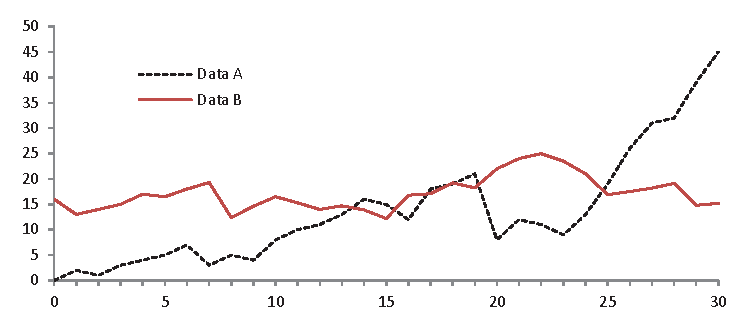
\includegraphics[width=\textwidth]{fig1.eps}
% \caption{A figure caption is always placed below the illustration.
% Please note that short captions are centered, while long ones are
% justified by the macro package automatically.} \label{fig1}
% \end{figure}
%
% \begin{theorem}
% This is a sample theorem. The run-in heading is set in bold, while
% the following text appears in italics. Definitions, lemmas,
% propositions, and corollaries are styled the same way.
% \end{theorem}
% %
% % the environments 'definition', 'lemma', 'proposition', 'corollary',
% % 'remark', and 'example' are defined in the LLNCS documentclass as well.
% %
% \begin{proof}
% Proofs, examples, and remarks have the initial word in italics,
% while the following text appears in normal font.
% \end{proof}
% For citations of references, we prefer the use of square brackets
% and consecutive numbers. Citations using labels or the author/year
% convention are also acceptable. The following bibliography provides
% a sample reference list with entries for journal
% articles~\cite{ref_article1}, an LNCS chapter~\cite{ref_lncs1}, a
% book~\cite{ref_book1}, proceedings without editors~\cite{ref_proc1},
% and a homepage~\cite{ref_url1}. Multiple citations are grouped
% \cite{ref_article1,ref_lncs1,ref_book1},
% \cite{ref_article1,ref_book1,ref_proc1,ref_url1}.

% \subsubsection{Acknowledgements} Please place your acknowledgments at
% the end of the paper, preceded by an unnumbered run-in heading (i.e.
% 3rd-level heading).

\subsubsection*{Acknowledgements}

I would like to thank my awesome graduate school supervisors, Dr. Amy Felty
and Dr. Philip Scott, as well as numerous colleagues at IOG,
for listening to me ramble on about this paradox.
I would especially like to thank Dr. Pieter Hofstra, may he rest in peace,
for making the bold move of asking for a resolution
of this paradox as a (surprise) bonus question on a computability theory exam.
I could not stop thinking about it ever since, until, hopefully, now.


% ---- Bibliography ----
%
% BibTeX users should specify bibliography style 'splncs04'.
% References will then be sorted and formatted in the correct style.

\bibliographystyle{splncs04}
\bibliography{hanging-bib}


\end{document}
